\documentclass{standalone}
\usepackage{tikz}
\usetikzlibrary{shapes.geometric, arrows, shapes.symbols}

\definecolor{mycolor}{RGB}{0, 153, 255}
\tikzstyle{process} = [rectangle, rounded corners,
                       minimum width=2cm, minimum height=1cm,
                       text centered, draw=black, fill=mycolor,
                       text=white, line width=0.3mm]

\tikzstyle{arrow} = [thick,->,>=stealth]

\begin{document}
    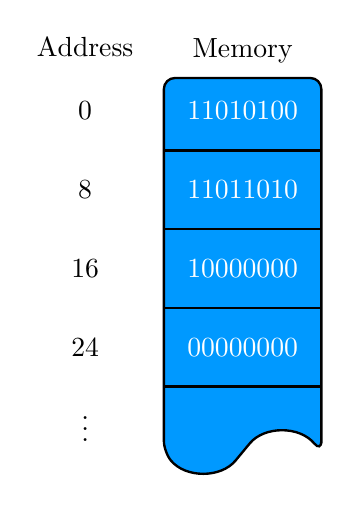
\begin{tikzpicture}[node distance=2cm]
        % Memory block
        \node at (0,2.6) [text centered] {Memory};
        \node at (0,0) [tape, rounded corners,
        minimum width=2cm, minimum height=5cm,
        text centered, draw=black, fill=mycolor,
        text=white, line width=0.3mm, tape bend top= none, tape bend height = 0.5 cm] {};
        
        % Lines in block
        \draw [line width=0.3mm] (-1,-1.67) -- (1,-1.67);
        \draw [line width=0.3mm] (-1,-0.67) -- (1,-0.67);
        \draw [line width=0.3mm] (-1,0.33) -- (1,0.33);
        \draw [line width=0.3mm] (-1,1.33) -- (1,1.33);
        
        % Data in blocks
        \node at (0,1.83) [text centered, text=white] {11010100}; %
        \node at (0,0.83) [text centered, text=white] {11011010}; %
        \node at (0,-0.17) [text centered, text=white] {10000000}; %
        \node at (0,-1.17) [text centered, text=white] {00000000}; %
        
        %Addresses
        \node at (-2,2.65) [text centered] {Address};
        \node at (-2,1.83) [text centered] {0};
        \node at (-2,0.83) [text centered] {8};
        \node at (-2,-0.17) [text centered] {16};
        \node at (-2,-1.17) [text centered] {24};
        \node at (-2,-2.1) [text centered] {$\vdots$};
    \end{tikzpicture}
\end{document}
